
\section{Zielsetung}
In diesem Versuch wird die Wärmeübertragung in Form der Wärmeleitung betrachtet.
Dabei werden die drei Metalle Aluminium, Messing und Edelstahl mit der statischen
und dynamische Methode untersucht.
\section{Theorie}
Bei einer nichtkonstante Temperaturverteilung entlang eines Körpers wird dieses
Ungleichgewicht durch ein Temperaturgefälle ausgeglichen. Dies kann durch Konvektion,
Wärmestrahlung oder Wärmeleitung passieren. Bei der Konvektion wird Wärme in Form von Materie
übertragen und bei der Wärmestrahlung durch elektromagnetische Wellen.
Die Wärmeleitung beruht auf dem Prinzip der Diffusion, wobei die Wärme über frei
bwegliche Elektronen weitergegeben wird, welche in diesem Versuch genauer betrachtet wird.
\newline
Bei der Betrachtung eines Stabes der Länge $L$ und der Querschnittsfläche $A$ gilt für die
zeitabhhänhige Wärmemenge $dQ$ folgender Zusammenhang
\begin{equation}
  dQ = -\kappa A \frac{\partial T}{\partial x}dt.
  \label{eqn:kappa}
\end{equation}
$\kappa$ ist hierbei die materialabhängig Wärmeleitfähigkeit. Das Minuszeichen in der Gleichung bedeutet,
dass der Wärmestrom vom wärmeren zum kälteren Teil des Stabes fließt.
Für die Wärmestromdichte $j_\text{w}$ gilt
\begin{equation}
  j_\text{w} = -\kappa \frac{\partial T}{\partial x} \, .
\end{equation}
Aus dieser kann mithilfe der Kontinuitätsgleichung die eindimensional Wellengleichung
\begin{equation}
  \frac{\partial T}{\partial t} = \frac{\kappa}{\rho c} \frac{\partial^2 T}{\partial x^2}
\end{equation}
formuliert werden.
\newline
Durch periodisches Erhitzen und Abkühlen eines langen Stabes breitet sich eine räumliche und zeitliche
Temperaturwelle
\begin{equation}
  T(x,t) = T_\text{max}\exp\left(-\sqrt{\frac{\omega \rho c}{2\kappa}}x\right) \cos\left(\omega t - \sqrt{\frac{\omega \rho c}{2\kappa}}x\right)
\end{equation}
in ihm aus, wobei
\begin{equation}
  v = \sqrt{\frac{2\omega \kappa}{\rho c}}.
\end{equation}
die Phasengeschwindkeit beschreibt.
\newline
Zur Berechnung des Dämpfungsfaktors der Welle werden die Amplituden $A_{nah}$ und $A_{fern}$ im Abstand
$\Delta{x}$ gemessen. Mit den Zusammenhänge $\omega = 2\pi /T^*$ und $\Phi = 2\pi \Delta{t}/T^*$
kann nun die Wärmeleitfähigkeit mit
\begin{equation}
  \kappa = \frac{\rho c (\symup{\Delta}x)^2}{2 \Delta{t} \ln(A_\text{nah}/A_\text{fern})}
  \label{eqn:kappa2}
\end{equation}
berechnet werden.
\section{Durchführung}
Der Versuch wird wie in Abbildung \ref{fig:aufbau} aufgebaut.
\newline
\begin{figure}[h]
  \centering
  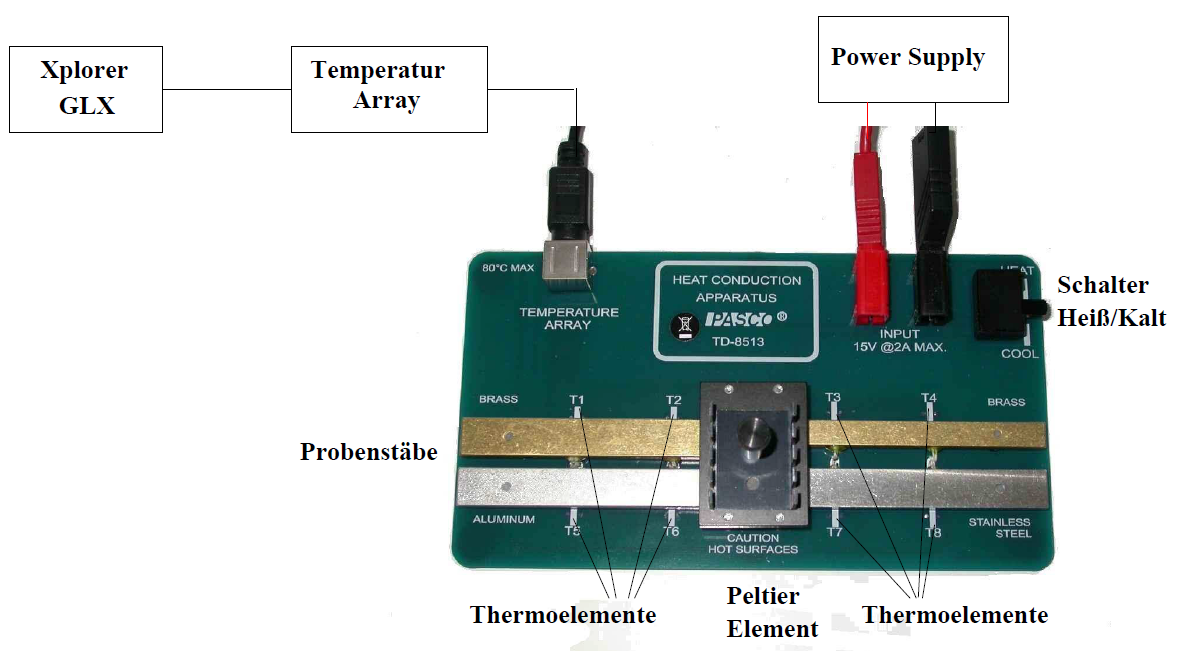
\includegraphics[scale=0.45]{aufbau.png}
  \caption{Versuchsaufbau.\cite{anleitung}}
  \label{fig:aufbau}
\end{figure}
\newline
Vor Beginn des Versuchs müssen zuerst die Verkabelungen überprüft werden. Zusätzlich ist es wichtig zu beachten,
dass die Wärmeisolierungen während des Versuchs über die Stäbe gelegt werden, damit möglichst wenig Wärme
mit der Umgebung ausgetauscht werden kann.
Die drei Messtäbe, für welche die Wärmeleitfähigkeit bestimmt werden sollen, werden durch das
Peltier-Element erhitzt und gekühlt. Dieses erzeugt eine Temperaturänderung bei Stromfluss.
Im Abstand von $\Delta{x}$ zweier Stellen auf dem Stab werden die Temperaturen mithilfe von
Thermoelementen gemessen. Über ein Temperatur-Array werden die Thermoelemente an einen Datenlogger
übertragen.
\newline
Nach jeder Messung werden die Wärmeisolierung entfernt und der Schalter auf 'COOL' gestellt, um die
Probestäbe zu kühlen.

\subsection{Statische Methode}
Bei der statischen Methode wird über den zeitlichen Temperaturverlauf an zwei gemessen Stellen auf
dem Stab die Wärmeleitfähigkeit bestimmt. Dafür wird die Abtastrate am Datenlogger auf $\Delta{t}=10\, \su{s}$
und am Power Supply bei maximalen Strom eine Spannung von $U_{P}=12.2\, \su{V}$ eingestellt. Erreicht das
Thermoelement T7 eine Temperatur von $45\si{\degreeCelsius}$ wird die Messung gestoppt.
\subsection{Dynamische Methode}
Bei der dynamischen Methode mit dem Angström-Messverfahren wird der Stab periodisch erwärmt und über die
Ausbreitungsgeschwindigkeit der Temperaturwelle die Wärmeleitfähigkeit bestimmt. Dafür wird die Abstastrate
am Datenlogger auf $\Delta{t}=2\, \su{s}$ und die Spannung auf $U_{P}=12.2\, \su{V}$ umgestellt. Der Stab wird dann
für 80\,s erhitzt und gekühlt. Dieses Verfahren wird für 10 Perioden durchgeführt.
\newline
Nach Abkühlung der Stäbe wird eine erneute Messung mit einer Periodendauer von 200\,s durchgeführt bis eines der
Thermoelemente eine Temperatur von $80\si{\degreeCelsius}$ erreicht hat.
